\chap{Summary of VPL Blocks}\label{a.blocks}

\sect{Event blocks}

\blksm{event-buttons} \textbf{Buttons}. Click on one or more of the images
of the buttons; they will turn red. An event will occur if the red
buttons are touched.

\bigskip\bigskip


\blksm{event-prox} \textbf{Horizontal sensors} (five at the front of the
Thymio and two at the back). Click on one or more of the small squares
and they will change color. Initially, all squares are gray, meaning
that the reading of each sensor is ignored.

If the square is white with a red border \blksm{center-prox}, an event
occurs if a lot of light is reflected.

If the square is black \blksm{center-no-prox}, an event occurs if little
light is reflected.

\bigskip

\trickbox{Ordinary objects need to be very close to the Thymio before they are
detected by the horizontal sensors. You can greatly increase
the range by attaching \emph{reflector tape}, such as used on bicycles,
to the objects.\footnote{My thanks to Francesco Mondada for showing this
to me!}\\
Compare the following image with \cref{fig.cat-mouse}:
\begin{center}
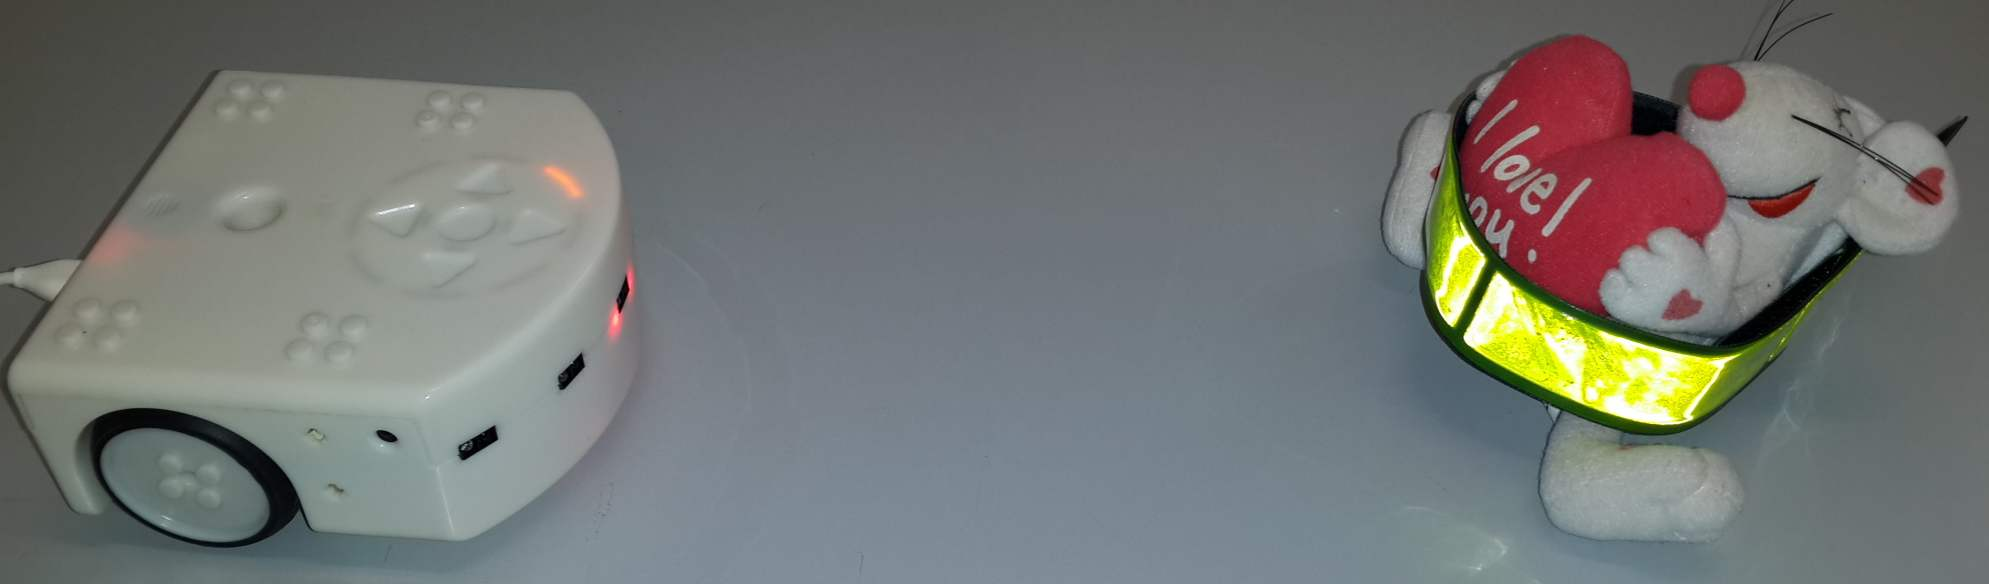
\includegraphics[width=0.8\textwidth]{reflect}
\end{center}
}

\bigskip

\blksm{event-ground} \textbf{Ground sensors} (two on the bottom of the
Thymio). Use like the block for the horizontal sensors.

\bigskip\bigskip

\blksm{event-prox-advanced}, \blksm{event-prox-ground-advanced}
\textbf{Sensors, advanced mode}. Use like the previous blocks. The top
slider sets the threshold above which an object is detected and the
bottom slider sets the threshold below which the absence of an object is
detected.

\bigskip\bigskip

There is an additional mode (the square is dark gray \blksm{slow-mid})
in which an event occurs if the value is between to upper and lower
threshold.

\bigskip\bigskip\bigskip

\blksm{event-tap} \textbf{Tap}. An event occurs when the Thymio is
tapped.

\bigskip\bigskip\bigskip

\blksm{event-tap-advanced} \textbf{Tap, advanced mode}. Use like the
previous block. Click on the small center or right circle to change to
an accelerometer event.

\bigskip\bigskip

\blksm{event-roll}, \blksm{event-pitch} \textbf{Accelerometer,
advanced mode}. Drag the white angle segment on the half-circle left or right.
An event will occur if the left / right or forwards / backwards angle
(respectively) of the Thymio is within the segment.

\bigskip\bigskip\bigskip\bigskip

\blksm{event-timer} \textbf{Timer, advanced mode}. An event occurs when
a timer has counted down to zero. The timer must have been set by a
previous timer \emph{action}.

\bigskip\bigskip\bigskip

\blksm{event-state} \textbf{State event, advanced mode}. The event
occurs only if the components of the current state match the
corresponding orange and white quarters of this block. The components
corresponding to the gray quarters need not match.

\bigskip

\sect{Action blocks}

\blksm{action-motors} \textbf{Motors}. Move the left and right sliders
up to increase the forwards rotation of the left and right motors,
respectively, and move the sliders down to increase the backwards
rotation.

\bigskip\bigskip

\blksm{action-colors-up} \textbf{Top lights}. Move the three sliders to
the right to increase the red, green and blue components of the top
light, respectively.

\bigskip\bigskip

\blksm{action-colors-down} \textbf{Bottom lights}. Turns the bottom
lights on. Use like the previous block.

\bigskip\bigskip\bigskip\bigskip

\blksm{action-music} \textbf{Music}. The six small circles are notes. A
black note is short and a white note is long. Click on a circle to
change the length. The five horizontal bars, represent tones. Click on
the bar to move a circle to that bar.

\bigskip\bigskip

\blksm{action-timer} \textbf{Timer, advanced mode} The timer can be set
for up to four seconds. Click anywhere within the white circle showing
the face of the clock. There will be a short animation and then the
amount of time until the alarm will be colored blue.

\bigskip\bigskip

\blksm{action-states} \textbf{States, advanced mode} The four
quarters in the block correspond to four components of a state.
Click a quarter to turn it to gray, orange or white.

\sect{Notes on the VPL Blocks}

\informationbox{Turning in place or a gentle turn}{When the motors run
at the same speed and in different directions, the robot turns in place.
However, if only one motor is on, the robot goes both forwards and in
the opposite direction. You may need to set a higher power to overcome
ground resistance.}

\informationbox{Rapid repetitive sensor events}{In most projects, you
set a color (white, black, dark gray) in a square in a sensor block to
indicate the the correspoding sensor participates in \emph{filtering}
the events. However, if \emph{all} the sensors remain in the original
gray, then no filtering is done. The event will occur 10 times per
second no matter what values are read from the sensors.}

\informationbox{Rapid repetitive button events}{The same holds true for
the button events, except that they occur 20 times per second.}
